\chapter{Introduction}
\begingroup
\setlength{\parindent}{0pt}
\setlength{\parskip}{0.5em}

Contract Central is a cloud-based mobile and web application designed to help users manage and understand their insurance-related documents. The platform leverages microservices, AI-powered document analysis, and semantic search to provide intuitive and intelligent access to contract information.

The key goals of Contract Central are:
\begin{itemize}
    \item To centralize the storage of administrative and insurance documents in a secure personal space.
    \item To assist users in understanding their contracts through natural language interaction.
    \item To detect redundant or overlapping coverage across different contracts.
    \item To answer common questions such as "Am I covered in case of theft?" or "What services are included with my credit card?"
\end{itemize}

The system is composed of multiple interconnected microservices, each responsible for a specific task in the processing pipeline. These services communicate asynchronously using Google Pub/Sub and are hosted on Google Cloud Platform.

The backend is divided into two main services:
\begin{itemize}
    \item \textbf{Data Management}: handles user authentication, file uploads, and Pub/Sub message orchestration.
    \item \textbf{Document Analysis}: processes files using Google Vertex AI and ChromaDB to enable semantic understanding and search.
\end{itemize}

On the client side, the application is developed with Flutter, allowing it to run seamlessly on both Android and iOS devices, as well as the web. The user interface supports uploading contracts, consulting AI-generated summaries, and querying coverage information via a conversational assistant.

By combining structured document storage, machine learning models, and a modern frontend, Contract Central aims to reduce the complexity of insurance management for everyday users.
\endgroup

\section{Overall Architecture}

The diagram below illustrates the overall architecture of Contract Central. It highlights the main components of the system and how they interact: the mobile/web frontend built with Flutter, the backend services running on Google Cloud, the use of Pub/Sub for asynchronous communication, and the integration of AI services such as Gemini and ChromaDB.

\begin{figure}[H]
    \centering
    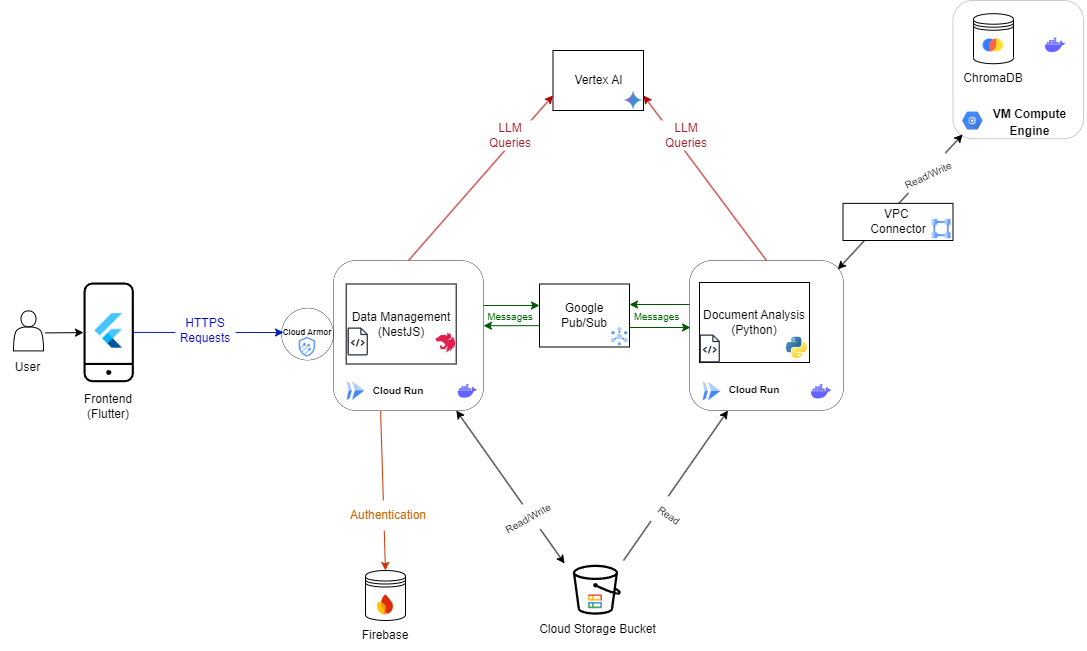
\includegraphics[width=0.95\textwidth]{architecture-contract-central.png}
    \caption{High-level architecture of the Contract Central platform}
    \label{fig:architecture}
\end{figure}